%%%%%%%%%%%%%%%%%%%%%%%%%%% asme2e.tex %%%%%%%%%%%%%%%%%%%%%%%%%%%%%%%
% Template for producing ASME-format articles using LaTeX            %
% Written by   Harry H. Cheng                                        %
%              Integration Engineering Laboratory                    %
%              Department of Mechanical and Aeronautical Engineering %
%              University of California                              %
%              Davis, CA 95616                                       %
%              Tel: (530) 752-5020 (office)                          %
%                   (530) 752-1028 (lab)                             %
%              Fax: (530) 752-4158                                   %
%              Email: hhcheng@ucdavis.edu                            %
%              WWW:   http://iel.ucdavis.edu/people/cheng.html       %
%              May 7, 1994                                           %
% Modified: February 16, 2001 by Harry H. Cheng                      %
% Modified: January  01, 2003 by Geoffrey R. Shiflett                %
% Use at your own risk, send complaints to /dev/null                 %
%%%%%%%%%%%%%%%%%%%%%%%%%%%%%%%%%%%%%%%%%%%%%%%%%%%%%%%%%%%%%%%%%%%%%%

%%% use twocolumn and 10pt options with the asme2e format
\documentclass[twocolumn,10pt]{asme2e}
\special{papersize=8.5in,11in}
\usepackage{amsmath}
\usepackage{tikz}
\usepackage{float}
\usepackage{pgfplots}
\usepackage{algorithm}
\usepackage{algorithmic}
\usepackage{bm}
\usepackage{cancel}
\usepackage{pgfplots}
%\usepackage{url}
\usepackage[obeyspaces]{url}
\usepackage{hyperref}
\usepackage{subcaption}

\usetikzlibrary{shapes,snakes, patterns}


%% The class has several options
%  onecolumn/twocolumn - format for one or two columns per page
%  10pt/11pt/12pt - use 10, 11, or 12 point font
%  oneside/twoside - format for oneside/twosided printing
%  final/draft - format for final/draft copy
%  cleanfoot - take out copyright info in footer leave page number
%  cleanhead - take out the conference banner on the title page
%  titlepage/notitlepage - put in titlepage or leave out titlepage
%  
%% The default is oneside, onecolumn, 10pt, final

%%% Replace here with information related to your conference
\confshortname{ME EN 6720 Semester Projects}
%\conffullname{the ASME 2009 International Design Engineering Technical Conferences \&\\
%              Computers and Information in Engineering Conference}

%%%%% for date in a single month, use
%\confdate{24-28}
%\confmonth{September}
%%%%% for date across two months, use
\confdate{April 29}
\confyear{2016}
\confcity{Salt Lake City}
\confcountry{USA}

%%% Replace DETC2009/MESA-12345 with the number supplied to you 
%%% by ASME for your paper.
%\papernum{ME EN 6720: Computational Fluid Dynamics}

%%% You need to remove 'DRAFT: ' in the title for the final submitted version.
\title{Use of the 2D Navier-Stokes Equations to Explore Aerodynamic Properties of Trains}

%%% first author
\author{Christopher E. Mertin
    \affiliation{
	School of Computing\\
	University of Utah\\
	Salt Lake City, Utah, 84112\\
    Email: \href{mailto:cmertin@cs.utah.edu}{cmertin@cs.utah.edu}
    }	
}


\begin{document}

\maketitle    

%%%%%%%%%%%%%%%%%%%%%%%%%%%%%%%%%%%%%%%%%%%%%%%%%%%%%%%%%%%%%%%%%%%%%%
\begin{abstract}
{\em This article explores the use of the 2D Incompressible Navier-Stokes Equations and their usefulness in determining the aerodynamic properties of train cars. This was accomplished by modeling the fluid flow around two rectangles with a variable distance between them and variable ground clearance, which is comparable to the air flow around and between train cars. By exploring this variable distance and ground clearance, the force exerted on the second train car can be calculated to see the effect on the train's aerodynamics.}
\end{abstract}

%%%%%%%%%%%%%%%%%%%%%%%%%%%%%%%%%%%%%%%%%%%%%%%%%%%%%%%%%%%%%%%%%%%%%%
\begin{nomenclature}
\entry{$u$}{\hspace{.15em}Non-dimensional horizontal velocity}
\entry{$v$}{\hspace{.15em}Non-dimensional vertical velocity}
\entry{$P$}{Pressure}
\entry{$\rho$}{Density}
\entry{$\nu$}{Kinematic Viscosity}
\entry{$\omega$}{\hspace{-.15em}Vorticity}
\entry{$R_{e}$}{\hspace{-.35em}Reynold's Number}
\end{nomenclature}

%%%%%%%%%%%%%%%%%%%%%%%%%%%%%%%%%%%%%%%%%%%%%%%%%%%%%%%%%%%%%%%%%%%%%%
\section*{INTRODUCTION}

The full Navier-Stokes Equations are used to determine the flow of viscous fluids. These equations come about from applying Newton's second law to fluid motion. 

There are two different formulations of these equations, those for {\em compressible flow} and those for {\em incompressible flow}. Compressible flow is where changes in the pressure of the temperature of the fluid cause changes in the density. If these changes in density are sufficiently small, these changes in density can be ignored and the fluid can be modeled as an incompressible flow.

In the instance of air, it can be treated as an incompressible fluid for speeds below Mach 0.3 \cite{incompressible}. The incompressible Navier-Stokes equations are represented as

\begin{align}
u\frac{\partial u}{\partial x} + v\frac{\partial u}{\partial y} + \frac{1}{\rho}\frac{\partial P}{\partial x} &= \nu\nabla^{2}u\\
u\frac{\partial u}{\partial x} + v\frac{\partial u}{\partial y} + \frac{1}{\rho}\frac{\partial P}{\partial y} &= \nu\nabla^{2}v
\intertext{with the continuity equation being}
\frac{\partial u}{\partial x} + \frac{\partial v}{\partial y} &= 0
\end{align}

With the appropriate boundary conditions, these are the equations that are to be solved for our system. With these results, it will be possible to tell which factors influence the amount of drag felt on the train cars the most.

%%%%%%%%%%%%%%%%%%%%%%%%%%%%%%%%%%%%%%%%%%%%%%%%%%%%%%%%%%%%%%%%%%%%%%
\section*{SOLVING THE NAVIER-STOKES EQUATIONS}

A full derivation of this algorithm can be seen in Appendix~A, which outlines the technique used to break up the 3 coupled PDEs stated above. It does so with the use of a temporary velocity variable (denoted as $\vec{u}^{(t)}$) by solving the equation with only the advection and diffusion terms. It then calculates the pressure needed to make the velocity field incompressible, and finally corrects the velocity by adding the pressure gradient.

The detailed algorithm with the equations can be seen in Algorithm~\ref{alg:navier_stokes}.

\begin{algorithm}[H]
\centering
\caption{Solving for the Primitive Variables\protect\footnotemark}
\begin{algorithmic}[1]
\WHILE{$\left|\left| P^{(n+1)} - P^{(n)}\right|\right|_{2} > tolerance$}
\STATE{Impose Boundary Conditions}
\STATE{$\vec{u}^{(t)} = \vec{u}^{(n)} + \Delta t \left(-\vec{A}^{(n)} + \vec{D}^{(n)}\right)$}
\STATE{$\nabla^{2}P^{(n+1)} = \frac{1}{\Delta t}\vec{\nabla}\cdot \vec{u}^{(t)}$}
\STATE{$\vec{u}^{(n+1)} = \vec{u}^{(t)} - \Delta t \nabla P^{(n+1)}$}
\STATE{$t = t + \Delta t$}
\ENDWHILE
\end{algorithmic}
\label{alg:navier_stokes}
\end{algorithm}

\footnotetext{{\tt C++} Code: \url{https://github.com/cmertin/CFD/proj2}\\ \hspace{5em}(Not yet uploaded)}

\subsubsection*{Parallelization}

The compute time for solving the Poisson Equation in Algorithm~\ref{alg:navier_stokes} can be greatly reduced by implementing a Parallel Gauss-Siedel Algorithm, which is also known as the ``Red-Black Gauss-Siedel'' \cite{redblack}.

%%%%%%%%%%%%%%%%%%%%%%%%%%%%%%%%%%%%%%%%%%%%%%%%%%%%%%%%%%%%%%%%%%%%%%
\section*{BOUNDARY CONDITIONS}

The boundary conditions used for solving this problem are typical, where the boundary conditions for the inlet and outlet can be seen in Figure~\ref{fig:grid}.

The ``ghost nodes'' exist to impose the boundary conditions on the domain and to make the computations easier. For the inlet and outlet, both Dirichlet and Von Neumann conditions are required.

In the case of the ghost nodes on the top and bottom of the domain, they were made periodic with the domain. In the creation of periodic boundary conditions, one grid in the $y$--direction is lost. However, the benefit that is gained is the domain is solved as an {\em infinite} domain.

\vspace{-1.5em}
\begin{figure}[H]
\centering
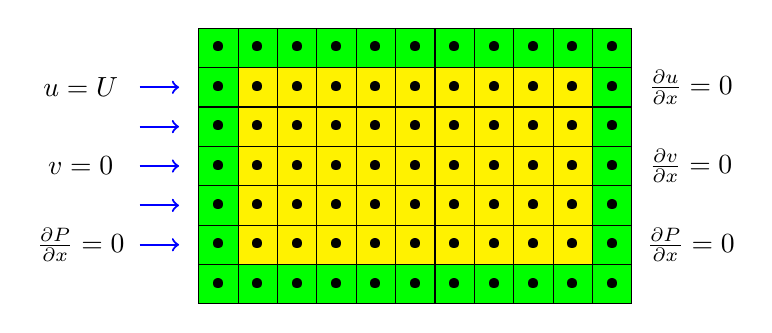
\begin{tikzpicture}[scale=0.5]
\draw[fill=green] (0,0) rectangle (11,7);
\draw[fill=yellow] (1,1) rectangle (10,6);
\draw (0,0) grid (11, 7);
\foreach \y in {0.5,...,6.5}
   \foreach \x in {0.5,...,10.5}
       \node at (\x,\y) {\textbullet};
\node at (12.5,5.5) {$\frac{\partial u}{\partial x} = 0$};
\node at (12.5,3.5) {$\frac{\partial v}{\partial x} = 0$};
\node at (12.5,1.5) {$\frac{\partial P}{\partial x} = 0$};
\node at (-3,5.5) {$u = U$};
\node at (-3,3.5) {$v = 0$};
\node at (-3,1.5) {$\frac{\partial P}{\partial x} = 0$};
\foreach \y in {1.5,...,5.5}
     \draw[blue,->,thick] (-1.5,\y) -- (-0.5,\y);
\end{tikzpicture}
\caption{Grid used in the computation. Green nodes denote the ``ghost nodes,'' while the yellow nodes cover the normal domain.}
\label{fig:grid}
\end{figure}

\subsubsection*{Boundary Conditions for Train Cars}
We also needed to impose boundary conditions on the train to satisfy the {\em no-slip condition}. The no-slip condition requires that viscous fluids will have no velocity relative to a solid boundary. Therefore, to impose these conditions, we set both $u$ and $v$ to be $0$ on the interior of the train cars, and the following on their boundaries:
\begin{itemize}
\item Left and Right Faces: $\frac{\partial u}{\partial x} = 0$ and $v = 0$
\item Top and Bottom Faces: $\frac{\partial v}{\partial y} = 0$ and $u = 0$
\end{itemize}

\section*{GRID TYPE}
The obvious choice of a grid is a collocated grid which stores $\{ P, u, v\}$ at each point in the grid. However, this causes problems with pressure--velocity coupling and the occurrence of oscillations in the pressure \cite{fergizer}. Instead, the use of the staggered grid was chosen to overcome these irregularities. A diagram for a single node of this staggered grid can be seen in Figure~\ref{fig:stagg_1}.
\vspace{-2em}
\begin{figure}[H]
\centering
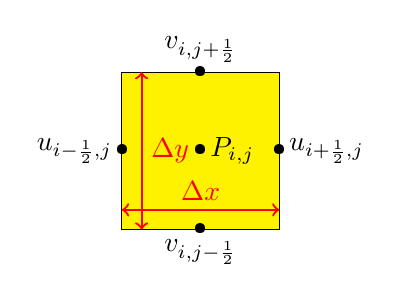
\begin{tikzpicture}[scale=0.5]
\draw [fill=yellow] (0, 0) rectangle (4,4);
\node at (0,2) {\textbullet};
\node at (2,2) {\textbullet};
\node at (4,2) {\textbullet};
\node at (2,0) {\textbullet};
\node at (2,4) {\textbullet};
\node [right] at (4,2) {$u_{i+\frac{1}{2},j}$};
\node [left] at (0,2) {$u_{i-\frac{1}{2},j}$};
\node [below] at (2,0) {$v_{i,j-\frac{1}{2}}$};
\node [above] at (2,4) {$v_{i,j+\frac{1}{2}}$};
\node [right] at (2,2) {$P_{i,j}$};
\node [right, red] at (0.5,2) {$\Delta y$};
\node [above, red] at (2,0.5) {$\Delta x$};
\draw [thick, red, <->] (0.5,0) -- (0.5,4);
\draw [thick, red, <->] (0, 0.5) -- (4, 0.5);
\end{tikzpicture}
\caption{Staggered Grid: Single Cell}
\label{fig:stagg_1}
\end{figure}



%%%%%%%%%%%%%%%%%%%%%%%%%%%%%%%%%%%%%%%%%%%%%%%%%%%%%%%%%%%%%%%%%%%%%%
\section*{VERIFICATION OF SIMULATION}

For simple problems, we can check to make sure that the code performs correctly. In doing so, we can derive an analytical solution for a simplified problem and test it for this case. We can do so using the {\em Reynold's Transport Theorem} \cite{Reynolds_Transport} which is stated as

\begin{align}
\frac{\text{d}B}{\text{d}t} &= \frac{\partial}{\partial t}\int_{C_{v}}\rho b \text{d}V + \int_{C_{s}}\rho b \vec{u}\cdot \text{d}\vec{s}
\intertext{where $B$ is any property of the local system. For the pressure, this equation turns into}
\frac{\text{d}P}{\text{d}t} = \sum \vec{F} &= \cancel{\frac{\partial}{\partial t}\int_{C_{v}}\rho \vec{u} \text{d}V} + \int_{C_{s}}\rho \vec{u}\left( \vec{u}\cdot \text{d}\vec{A}\right)\label{eq:full_p}
\intertext{with the first term going to zero due to conservation of flux. The forces that the train car are going to experience are the pressure $(F_{p})$, the lift force $(F_{L})$, and the drag force $(F_{d})$. $F_{p}$ and $F_{L}$ are defined as}
F_{p} &= -\int p\ \text{d}\vec{A}\label{eq:F_p}\\
F_{L} &= \oint p \cdot \hat{n}\ \text{d}A\label{eq:F_l}
\intertext{where we can rearrange Equation~(\ref{eq:full_p}) to solve for $F_{d}$, giving}
F_{d} &= \int p\ \text{d}\vec{A} - \oint p \cdot \hat{n}\ \text{d}A + \int_{C_{s}}\rho \vec{u}\left( \vec{u}\cdot \text{d}\vec{A}\right)\label{eq:drag}
\end{align}

Using Equation~(\ref{eq:drag}), we can calculate the drag force by creating the correct {\em control volume} to contain the box. The simpliest case was for the flow around a simple square. For the analytical solution, we can use the following drag equation:

\begin{align}
F_{d} &= \frac{1}{2}\rho u^{2} C_{D} A\label{eq:fd}
\end{align}

where $C_{D}$ is the drag coefficient and $A$ is the cross-sectional area. For a simple square or cube, $C_{D}=2.2$ \cite{drag_force}. In the code for the rest of the paper, $\rho = 1$ which is what was used to develop the algorithm. In order to verify that the results were correct, various values of $u$ for Equation~(\ref{eq:fd}) and Equation~(\ref{eq:drag}).

There are multiple types of drag forces that influence how the square behaves in the flow. For example:

\begin{itemize}
\item {\bf Induced Drag:} Drag resulting from trailing vortex
\item {\bf Skin Friction Drag:} Drag on the body over its contact surface
\item {\bf Form Drag:} The drag on a body resulting on the pressure acting on the normal to the body's surface
\end{itemize}

Therefore, to account for all these forms of drag, the control volume that was made was to contain the {\em entire} surface of the block. The results for this can be seen in Figure~\ref{fig:p_vs_v} where the values for $F_{d}$ were calculated {\em exactly} and from the {\em control volume} approach. Figure~\ref{fig:p_error} shows the error for the different runs, which shows that the error was approximately $3.3\%$ for each of the simulations. This could have been reduced even further by using a finer discritization of the domain, however the computation time was more important than correcting a $3.3\%$ error.


\begin{figure}[h]
\centering
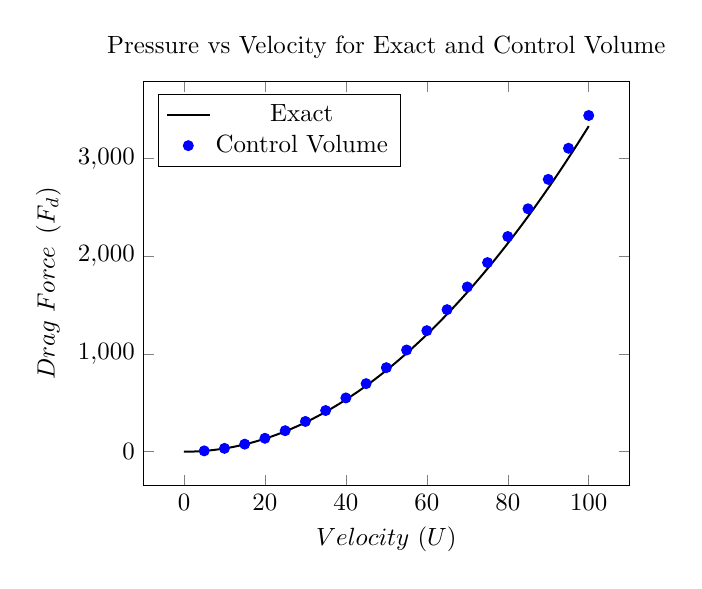
\begin{tikzpicture}[scale=.9]%[scale = 0.75]
\begin{axis}[xlabel={$Velocity\ (U)$}, ylabel={$Drag\ Force\ \left(F_{d}\right)$}, legend pos=north west, title={Pressure vs Velocity for Exact and Control Volume}]
\addplot[thick, color=black] coordinates{(0,0.000)(1,0.333)(2,1.333)(3,3.000)(4,5.333)(5,8.333)(6,12.000)(7,16.333)(8,21.333)(9,27.000)(10,33.333)(11,40.333)(12,48.000)(13,56.333)(14,65.333)(15,75.000)(16,85.333)(17,96.333)(18,108.000)(19,120.333)(20,133.333)(21,147.000)(22,161.333)(23,176.333)(24,192.000)(25,208.333)(26,225.333)(27,243.000)(28,261.333)(29,280.333)(30,300.000)(31,320.333)(32,341.333)(33,363.000)(34,385.333)(35,408.333)(36,432.000)(37,456.333)(38,481.333)(39,506.999)(40,533.333)(41,560.333)(42,587.999)(43,616.333)(44,645.333)(45,674.999)(46,705.333)(47,736.333)(48,767.999)(49,800.333)(50,833.333)(51,866.999)(52,901.332)(53,936.332)(54,971.999)(55,1008.332)(56,1045.332)(57,1082.999)(58,1121.332)(59,1160.332)(60,1199.999)(61,1240.332)(62,1281.332)(63,1322.999)(64,1365.332)(65,1408.332)(66,1451.999)(67,1496.332)(68,1541.332)(69,1586.998)(70,1633.332)(71,1680.332)(72,1727.998)(73,1776.332)(74,1825.332)(75,1874.998)(76,1925.331)(77,1976.331)(78,2027.998)(79,2080.331)(80,2133.331)(81,2186.998)(82,2241.331)(83,2296.331)(84,2351.998)(85,2408.331)(86,2465.331)(87,2522.997)(88,2581.331)(89,2640.331)(90,2699.997)(91,2760.331)(92,2821.331)(93,2882.997)(94,2945.330)(95,3008.330)(96,3071.997)(97,3136.330)(98,3201.330)(99,3266.997)(100,3333.330)};
\addlegendentry{Exact}
\addplot[color=blue, mark=*, only marks] coordinates{(5,8.608)(10,34.429)(15,77.464)(20,137.714)(25,215.178)(30,309.856)(35,421.748)(40,550.854)(45,697.174)(50,860.709)(55,1041.457)(60,1239.420)(65,1454.597)(70,1686.988)(75,1936.594)(80,2203.413)(85,2487.447)(90,2788.695)(95,3107.157)(100,3442.833)};
\addlegendentry{Control Volume}
\end{axis}
\end{tikzpicture}
\caption{Plot of the Pressure vs the Velocity on a single block}
\label{fig:p_vs_v}
\end{figure}

\begin{figure}[h]
\centering
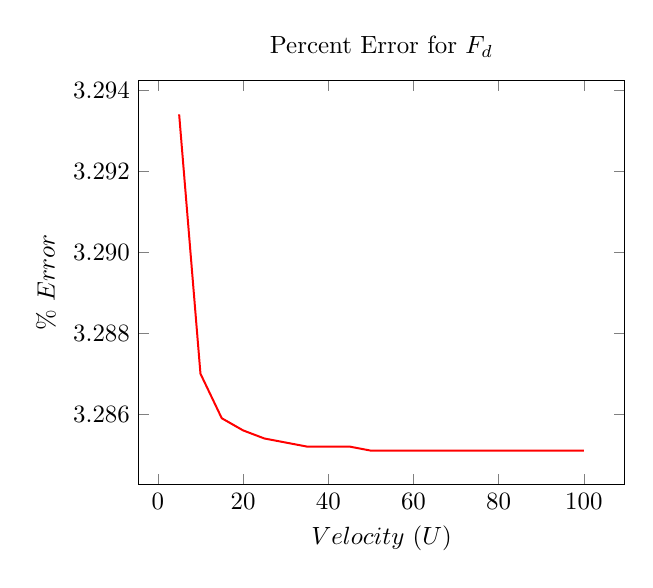
\begin{tikzpicture}[scale=.9]%[scale = 0.75]
\begin{axis}[xlabel={$Velocity\ (U)$}, ylabel={$\%\ Error$}, legend pos=north east, title={Percent Error for $F_{d}$}, y tick label style={/pgf/number format/.cd,fixed,fixed zerofill,precision=3,/tikz/.cd}]
\addplot[thick, color=red] coordinates{(5,3.2934)(10,3.2870)(15,3.2859)(20,3.2856)(25,3.2854)(30,3.2853)(35,3.2852)(40,3.2852)(45,3.2852)(50,3.2851)(55,3.2851)(60,3.2851)(65,3.2851)(70,3.2851)(75,3.2851)(80,3.2851)(85,3.2851)(90,3.2851)(95,3.2851)(100,3.2851)};
\end{axis}
\end{tikzpicture}
\caption{Plot of the Percent Error from the simulation}
\label{fig:p_error}
\end{figure}

\begin{figure}[h]
\centering
\includegraphics[width=.4\textwidth]{figs/pressure_single.pdf}
\caption{Typical plot for the pressure around a single block with $U=10$}
\end{figure}

\begin{figure}[h]
\centering
\includegraphics[width=.4\textwidth]{figs/vorticity_single.pdf}
\caption{Typical plot of vorticity and streamfunction around a single block with $U=10$}
\end{figure}

In Figure~\ref{fig:p_error}, the change in error is most likely due to the change in the time step, $\Delta t$, which is calculated in relation to the velocity with the following relation

\begin{align}
\Delta t = \frac{(\Delta x)^{2}}{40\nu}\label{eq:dt}
\end{align}

\noindent which is scaled by a factor of $10$ for the bounds. Where $\nu\propto u$



\section*{RESULTS}

In order to get the correct results, various experiments were performed with different parameters. From Equation~(\ref{eq:fd}) and Figure~\ref{fig:p_vs_v}, it is easy to see that the pressure imparted the ``train car'' is proportional to the square of the velocity. However, there are other parameters that need to be looked at as well. For example, the spacing between the train cars, and the diameter of the wheels, {\em i.e.} ground clearance.

As we know what $F_{d}$ is for a single block, it was more interesting to look at $\Delta F_{d}$, which is $F_{d}$ from the control volume on the second train car from Equation~(\ref{eq:fd}) minus $F_{d}$ from Equation~(\ref{eq:drag}) for a single block. This makes it easy to see the variations between the train car and the single block.

\subsubsection*{Spacing Between Cars}

In testing the spacing between the cars, $\Delta F_{d}$ should change relative to the velocity. Therefore, 4 different instances of $U$ were tested with various separation distances, which can be seen in Figure~\ref{fig:fd_sub}. This plot shows the difference between $F_{d}$ on the second train car and $F_{d}$ experienced by the single block.

As the size of the blocks are the same, the {\em skin friction drag} should be the same in each case. Therefore, when calculating $\Delta F_{d}$, the value should only be the form drag that is experienced on the block as everything else is equal. As these results show, the largest change in $F_{d}$ experienced by the second car was when there was minimal spacing between the two. As expected, as the spacing increased, the change in the drag force decreased. Due to computational limits on time, only up to $5/3$ of the ratio between the separation and the width of the train car could be computed. In theory, there is some distance to place the second train car such that it will not experience any effects from the first train car and will behave as a standalone block.

However, there seems to have been a ``limit'' that was reached as the change in $F_{d}$ trailed off. This is also seen in Figure~\ref{fig:fd_ratio} which compares the ratio of $F_{d}$ from the second train car to that of a single block. The overall change in $F_{d}$ on the second car was no more than a $1.0\%$ increase at the most, and trailed off to a $0.4\%$ increase. This trailing off in change is likely due to reaching the limits of the domain, where the range of values were restricted due to the boundary conditions.

\begin{figure}[h]
\centering
\includegraphics[width=.4\textwidth]{figs/pressure_sep.pdf}
\caption{Pressure on the train for $U=10$ and $separation/width=11/15$}
\label{fig:p_sep}
\end{figure}

Figure~\ref{fig:fd_ratio} shows that the dependence on the velocity can be removed with a simple ratio of the two as $F_{d}^{(sep)}$ and $F_{d}$ had the same values for each of the simulations. Therefore, when testing the ground clearance, computational time can be saved by only running for a single value of $U$ and plotting the ratio between the two values instead.

\begin{figure}[h]
\centering
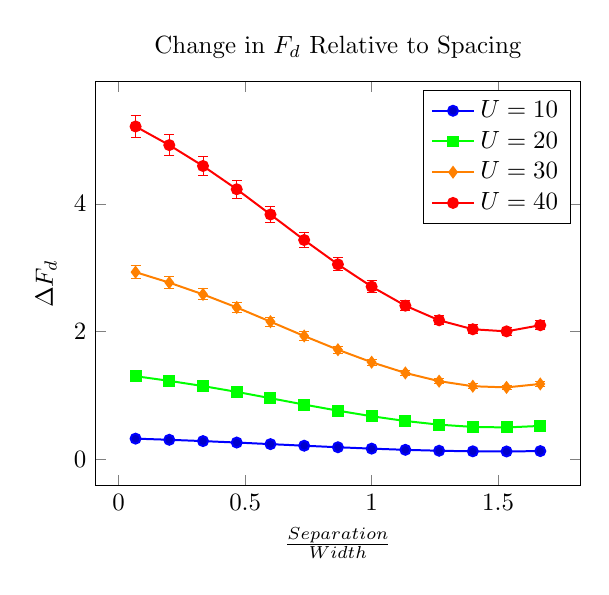
\begin{tikzpicture}[scale=.9]
\begin{axis}[xlabel={$\frac{Separation}{Width}$}, ylabel={$\Delta F_{d}$}, title = {Change in $F_{d}$ Relative to Spacing}]
\addplot+[thick, error bars/.cd, y dir=both, y explicit] coordinates{
(0.0667,0.3262) +- (0.0108,0.0108)
(0.2000,0.3081) +- (0.0102,0.0102)
(0.3333,0.2877) +- (0.0095,0.0095)
(0.4667,0.2650) +- (0.0087,0.0087)
(0.6000,0.2403) +- (0.0079,0.0079)
(0.7333,0.2153) +- (0.0071,0.0071)
(0.8667,0.1915) +- (0.0063,0.0063)
(1.0000,0.1696) +- (0.0056,0.0056)
(1.1333,0.1510) +- (0.0050,0.0050)
(1.2667,0.1366) +- (0.0045,0.0045)
(1.4000,0.1277) +- (0.0042,0.0042)
(1.5333,0.1255) +- (0.0041,0.0041)
(1.6667,0.1313) +- (0.0043,0.0043)
};
\addlegendentry{$U = 10$}
\addplot+[color=green, mark=square*, mark options=green, thick, error bars/.cd, y dir=both, y explicit] coordinates{
(0.0667,1.3030) +- (0.0430,0.0430)
(0.2000,1.2302) +- (0.0406,0.0406)
(0.3333,1.1485) +- (0.0379,0.0379)
(0.4667,1.0575) +- (0.0349,0.0349)
(0.6000,0.9587) +- (0.0316,0.0316)
(0.7333,0.8589) +- (0.0283,0.0283)
(0.8667,0.7637) +- (0.0252,0.0252)
(1.0000,0.6765) +- (0.0223,0.0223)
(1.1333,0.6020) +- (0.0199,0.0199)
(1.2667,0.5448) +- (0.0180,0.0180)
(1.4000,0.5095) +- (0.0168,0.0168)
(1.5333,0.5012) +- (0.0165,0.0165)
(1.6667,0.5252) +- (0.0173,0.0173)
};
\addlegendentry{$U = 20$}
\addplot+[color=orange, mark=diamond*, mark options=orange, thick, error bars/.cd, y dir=both, y explicit] coordinates{
(0.0667,2.9310) +- (0.0967,0.0967)
(0.2000,2.7670) +- (0.0913,0.0913)
(0.3333,2.5832) +- (0.0852,0.0852)
(0.4667,2.3785) +- (0.0785,0.0785)
(0.6000,2.1562) +- (0.0712,0.0712)
(0.7333,1.9317) +- (0.0637,0.0637)
(0.8667,1.7174) +- (0.0567,0.0567)
(1.0000,1.5214) +- (0.0502,0.0502)
(1.1333,1.3539) +- (0.0447,0.0447)
(1.2667,1.2252) +- (0.0404,0.0404)
(1.4000,1.1460) +- (0.0378,0.0378)
(1.5333,1.1276) +- (0.0372,0.0372)
(1.6667,1.1816) +- (0.0390,0.0390)
};
\addlegendentry{$U = 30$}
\addplot+[color=red, mark=oplus*, thick, error bars/.cd, y dir=both, y explicit] coordinates{
(0.0667,5.2102) +- (0.1719,0.1719)
(0.2000,4.9187) +- (0.1623,0.1623)
(0.3333,4.5919) +- (0.1515,0.1515)
(0.4667,4.2279) +- (0.1395,0.1395)
(0.6000,3.8328) +- (0.1265,0.1265)
(0.7333,3.4337) +- (0.1133,0.1133)
(0.8667,3.0527) +- (0.1007,0.1007)
(1.0000,2.7042) +- (0.0892,0.0892)
(1.1333,2.4065) +- (0.0794,0.0794)
(1.2667,2.1778) +- (0.0719,0.0719)
(1.4000,2.0372) +- (0.0672,0.0672)
(1.5333,2.0044) +- (0.0661,0.0661)
(1.6667,2.1005) +- (0.0693,0.0693)
};
\addlegendentry{$U = 40$}
\end{axis}
\end{tikzpicture}
\caption{Plot of $F_{d}$ experienced by the second train car subtracted from $F_{d}$ on a single block}
\label{fig:fd_sub}
\end{figure}

\begin{figure}[h]
\centering
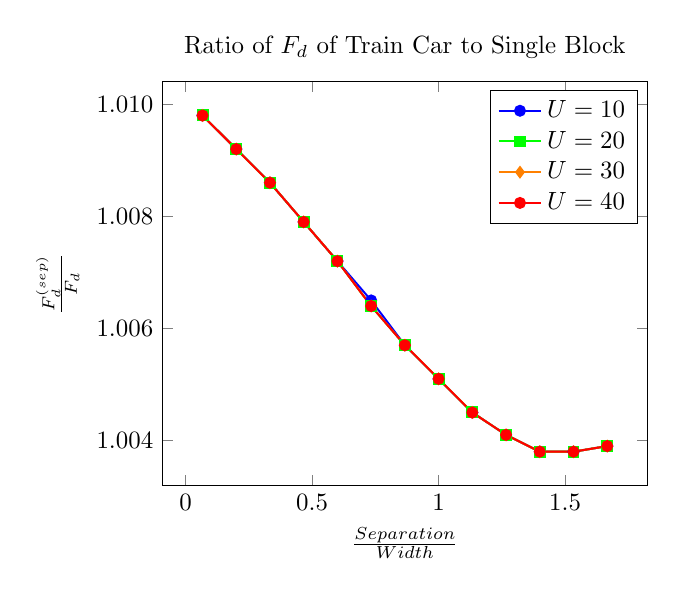
\begin{tikzpicture}[scale=.9]
\begin{axis}[xlabel={$\frac{Separation}{Width}$}, ylabel={$\frac{F_{d}^{(sep)}}{F_{d}}$}, title={Ratio of $F_{d}$ of Train Car to Single Block}, y tick label style={/pgf/number format/.cd,fixed,fixed zerofill,precision=3,/tikz/.cd}]
\addplot[mark=*, thick, color=blue] coordinates{
(0.0667,1.0098)
(0.2000,1.0092)
(0.3333,1.0086)
(0.4667,1.0079)
(0.6000,1.0072)
(0.7333,1.0065)
(0.8667,1.0057)
(1.0000,1.0051)
(1.1333,1.0045)
(1.2667,1.0041)
(1.4000,1.0038)
(1.5333,1.0038)
(1.6667,1.0039)
};
\addlegendentry{$U = 10$}
\addplot[mark=square*, thick, color=green] coordinates{
(0.0667,1.0098)
(0.2000,1.0092)
(0.3333,1.0086)
(0.4667,1.0079)
(0.6000,1.0072)
(0.7333,1.0064)
(0.8667,1.0057)
(1.0000,1.0051)
(1.1333,1.0045)
(1.2667,1.0041)
(1.4000,1.0038)
(1.5333,1.0038)
(1.6667,1.0039)
};
\addlegendentry{$U = 20$}
\addplot[mark=diamond*, thick, color=orange] coordinates{
(0.0667,1.0098)
(0.2000,1.0092)
(0.3333,1.0086)
(0.4667,1.0079)
(0.6000,1.0072)
(0.7333,1.0064)
(0.8667,1.0057)
(1.0000,1.0051)
(1.1333,1.0045)
(1.2667,1.0041)
(1.4000,1.0038)
(1.5333,1.0038)
(1.6667,1.0039)
};
\addlegendentry{$U = 30$}
\addplot[mark=otimes*, thick, color=red] coordinates{
(0.0667,1.0098)
(0.2000,1.0092)
(0.3333,1.0086)
(0.4667,1.0079)
(0.6000,1.0072)
(0.7333,1.0064)
(0.8667,1.0057)
(1.0000,1.0051)
(1.1333,1.0045)
(1.2667,1.0041)
(1.4000,1.0038)
(1.5333,1.0038)
(1.6667,1.0039)
};
\addlegendentry{$U = 40$}
\end{axis}
\end{tikzpicture}
\caption{Ratio between $F_{d}$ on the second train car to that of $F_{d}$ experienced on a single block}
\label{fig:fd_ratio}
\end{figure}

\subsubsection*{Ground Clearance}
For the second car, the ``midpoint'' of the separation of the previous section was chosen. This was chosen arbitrary just to see how the height effects the train car. The separation distance over the width of the train car that was chosen was $11/15$. As the separation is being kept constant, the results from this experiment should be applicable to other separations.

\begin{figure}[h]
\centering
\includegraphics[width=.4\textwidth]{figs/pressure_clearance.pdf}
\caption{Pressure on train for $U=10$ and $clearance/width = 1/3$}
\label{fig:clearance}
\end{figure}

The results from this can be seen in Figure~\ref{fig:fdclear_fd}, show that the {\em optimal} ground clearance occurs at $1/15$, the smallest ground clearance. At this point, $F_{d}$ is approximately $25\%$ of the value for a single block. This ratio would be similar when compared to $F_{d}^{(sep)}$ since $F_{d}^{(sep)}/F_{d}\approx 1$. 

The large jump near the end of the results is most likely due to approaching the domain boundaries. As is shown in the figure, it never approaches the value of a single block.

\begin{figure}[h]
\centering
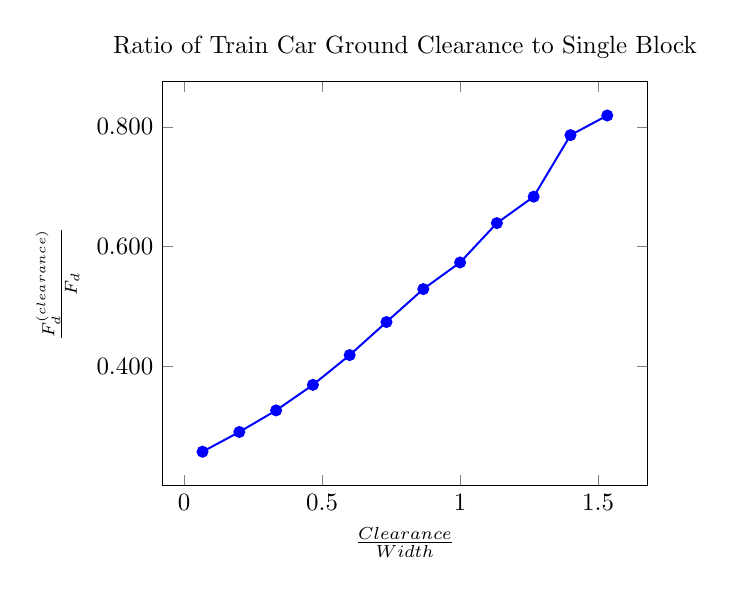
\begin{tikzpicture}[scale=.9]
\begin{axis}[xlabel={$\frac{Clearance}{Width}$}, ylabel={$\frac{F_{d}^{(clearance)}}{F_{d}}$}, title={Ratio of Train Car Ground Clearance to Single Block}, y tick label style={/pgf/number format/.cd,fixed,fixed zerofill,precision=3,/tikz/.cd}]
\addplot[mark=*, thick, color=blue] coordinates{
(0.0667,0.2568)
(0.2000,0.2898)
(0.3333,0.3259)
(0.4667,0.3686)
(0.6000,0.4184)
(0.7333,0.4737)
(0.8667,0.5288)
(1.0000,0.5733)
(1.1333,0.6391)
(1.2667,0.6833)
(1.4000,0.7862)
(1.5333,0.8191)
};
%\addlegendentry{$U = 10$}
\end{axis}
\end{tikzpicture}
\caption{Ratio of $F_{d}$ experienced on the second train car to that of a single block with $separation/width = 11/15$}
\label{fig:fdclear_fd}
\end{figure}

\section*{CONCLUSION}

The largest change in the drag force came from the ground clearance of the train. There was a minimal contribution from the spacing between the train cars, with a maximum change of only $1\%$ which decreased to a change of $0.4\%$ as the separation approached $5/3$ of $separation/width$ of the train car.

In the case of the ground clearance, the best instance was for the train being closer to the ground with resulted in a $75\%$ reduction in $F_{d}$ which tappered off to approximately a $20\%$ reduction towards the end of the scale.

The results of these experiments were not surprising in the case of the ground clearance, as the lower to the ground the higher the $F_{L}$. And from Equation~(\ref{eq:drag}) it should make $F_{d}$ smaller. However, the minimal changes in $F_{d}$ due to separation was infact surprising, showing that there was no large differences to worry about when building a train as such. Therefore, to make a train ``more stable,'' shorter distances between train cars can be used to minimize material cost. 

On top of this, as the ground clearance was an important factor as well, it turned out that the smaller the wheels the better aerodynamic properties of the train as well. Therefore, minimizing the diameter of the train wheels was important not only in manufacturing costs of the train, but also in helping with the train's aerodynamics. Thus, the best train to build in a cost and aerodynamics standpoint would be to have short distances between the train cars and also give it the lowest ground clearance possible.

%%%%%%%%%%%%%%%%%%%%%%%%%%%%%%%%%%%%%%%%%%%%%%%%%%%%%%%%%%%%%%%%%%%%%%
%\section*{FOOTNOTES\protect\footnotemark}
%\footnotetext{Examine the input file, asme2e.tex, to see how a footnote is given in a head.}
%Footnotes are referenced with superscript numerals and are numbered consecutively from 1 to the end of the paper\footnote{Avoid footnotes if at all possible.}. Footnotes should appear at the bottom of the column in which they are referenced.
%%%%%%%%%%%%%%%%%%%%%%%%%%%%%%%%%%%%%%%%%%%%%%%%%%%%%%%%%%%%%%%%%%%%%%

% Here's where you specify the bibliography style file.
% The full file name for the bibliography style file 
% used for an ASME paper is asmems4.bst.




%%%%%%%%%%%%%%%%%%%%%%%%%%%%%%%%%%%%%%%%%%%%%%%%%%%%%%%%%%%%%%%%%%%%%%
%\begin{acknowledgment}
%Special thanks to Donald Trump for Making~America~Great~Again.
%\end{acknowledgment}

%%%%%%%%%%%%%%%%%%%%%%%%%%%%%%%%%%%%%%%%%%%%%%%%%%%%%%%%%%%%%%%%%%%%%%
% The bibliography is stored in an external database file
% in the BibTeX format (file_name.bib).  The bibliography is
% created by the following command and it will appear in this
% position in the document. You may, of course, create your
% own bibliography by using thebibliography environment as in
%
% \begin{thebibliography}{12}
% ...
% \bibitem{itemreference} D. E. Knudsen.
% {\em 1966 World Bnus Almanac.}
% {Permafrost Press, Novosibirsk.}
% ...
% \end{thebibliography}

% Here's where you specify the bibliography database file.
% The full file name of the bibliography database for this
% article is asme2e.bib. The name for your database is up
% to you.
\ \newpage
\bibliographystyle{asmems4}
\bibliography{bibliography}

%%%%%%%%%%%%%%%%%%%%%%%%%%%%%%%%%%%%%%%%%%%%%%%%%%%%%%%%%%%%%%%%%%%%%%
\appendix       %%% starting appendix
\section*{Appendix A: DERIVATION OF ALGORITHM \ref{alg:navier_stokes}}\label{derivation}
The Navier-Stokes Equations need to satisfy the constraints of {\em Conservation of Mass} and {\em Conservation of Momentum}, where the equations are derived below.

\noindent{\bf  Conservation of Mass}
To solve the system while conserving mass, the grid that was used was the staggered grid which can be seen in Figure~\ref{fig:stagg_1}. To conserve mass in the element, the following needs to be satisfied

\begin{align}
\oint_{s}\vec{u}\cdot \hat{n} \text{ d}s = 0
\end{align}

which simply states that the flow of the velocity in each component of the system. If we integrate over this boundary, and with $h = \Delta x = \Delta y$, we get

\begin{align}
hu_{i+\frac{1}{2},j}^{(n+1)} - hu_{i-\frac{1}{2},j}^{(n+1)} + hv_{i,j+\frac{1}{2}}^{(n+1)} - hv_{i,j-\frac{1}{2}}^{(n+1)} = 0
\intertext{where, if we divide by $h$ gives us}
u_{i+\frac{1}{2},j}^{(n+1)} - u_{i-\frac{1}{2},j}^{(n+1)} + v_{i,j+\frac{1}{2}}^{(n+1)} - v_{i,j-\frac{1}{2}}^{(n+1)} = 0
\end{align}
\noindent{\bf  Conservation of Momentum: Advection Terms}

For the momenum conservation, we can define the control volumes for $u$ and $v$ as seen in Figure~\ref{fig:stagg_u} and Figure~\ref{fig:stagg_v}. To find the momenum conservation, we need to define the cell averages. The elements of each cell are defined in Figure~\ref{fig:avg}.

\begin{figure}[H]
\centering
\begin{minipage}{.4\textwidth}
\centering
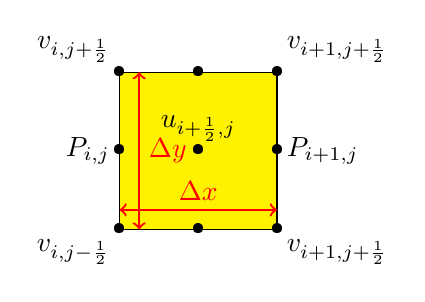
\begin{tikzpicture}[scale = 0.5]
\draw [fill=yellow] (0, 0) rectangle (4,4);
\foreach \x in {0,2,4}
    \foreach \y in {0,2,4}
        \node at (\x,\y) {\textbullet};

\node [right] at (4,2) {$P_{i+1,j}$};
\node [left] at (0,2) {$P_{i,j}$};
\node [above left] at (0,4) {$v_{i,j+\frac{1}{2}}$};
\node [above right] at (4,4) {$v_{i+1,j+\frac{1}{2}}$};
\node [below left] at (0,0) {$v_{i,j-\frac{1}{2}}$};
\node [below right] at (4,0) {$v_{i+1,j+\frac{1}{2}}$};
\node [above] at (2,2) {$u_{i+\frac{1}{2},j}$};
\node [right, red] at (0.5,2) {$\Delta y$};
\node [above, red] at (2,0.5) {$\Delta x$};
\draw [thick, red, <->] (0.5,0) -- (0.5,4);
\draw [thick, red, <->] (0, 0.5) -- (4, 0.5);
\end{tikzpicture}
\captionof{figure}{Control Volume for $u$}
\label{fig:stagg_u}
\end{minipage}
\hspace{5em}
\begin{minipage}{.4\textwidth}
\centering
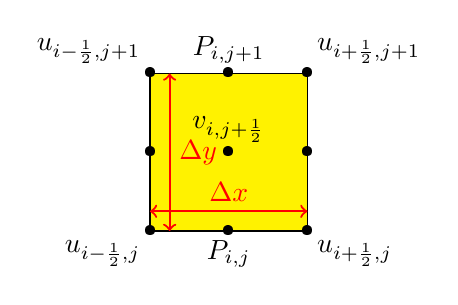
\begin{tikzpicture}[scale = 0.5]
\draw [fill=yellow] (0, 0) rectangle (4,4);
\foreach \x in {0,2,4}
    \foreach \y in {0,2,4}
        \node at (\x,\y) {\textbullet};

\node [above] at (2,4) {$P_{i,j+1}$};
\node [below] at (2,0) {$P_{i,j}$};
\node [above left] at (0,4) {$u_{i-\frac{1}{2},j+1}$};
\node [above right] at (4,4) {$u_{i+\frac{1}{2},j+1}$};
\node [below left] at (0,0) {$u_{i-\frac{1}{2},j}$};
\node [below right] at (4,0) {$u_{i+\frac{1}{2},j}$};
\node [above] at (2,2) {$v_{i,j+\frac{1}{2}}$};
\node [right, red] at (0.5,2) {$\Delta y$};
\node [above, red] at (2,0.5) {$\Delta x$};
\draw [thick, red, <->] (0.5,0) -- (0.5,4);
\draw [thick, red, <->] (0, 0.5) -- (4, 0.5);
\end{tikzpicture}
\captionof{figure}{Control Volume for $v$}
\label{fig:stagg_v}
\end{minipage}
\end{figure}

\begin{figure}[H]
\centering
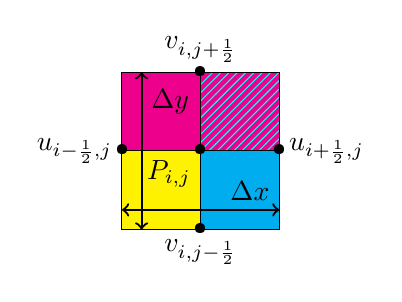
\begin{tikzpicture}[scale = 0.5]
\draw [fill=yellow] (0, 0) rectangle (4,4);
\draw [fill=cyan] (2,0) rectangle(4,2);
\draw [fill=magenta] (0,2) rectangle(4,4);
\draw [pattern = north east lines, pattern color=cyan] (2,2) rectangle(4,4);
\node at (0,2) {\textbullet};
\node at (2,2) {\textbullet};
\node at (4,2) {\textbullet};
\node at (2,0) {\textbullet};
\node at (2,4) {\textbullet};
%\draw[fill] (0,2) circle[radius=0.05];
%\draw[fill] (2,2) circle[radius=0.05];
%\draw[fill] (4,2) circle[radius=0.05];
%\draw[fill] (2,0) circle[radius=0.05];
%\draw[fill] (2,4) circle[radius=0.05];
\node [right] at (4,2) {$u_{i+\frac{1}{2},j}$};
\node [left] at (0,2) {$u_{i-\frac{1}{2},j}$};
\node [below] at (2,0) {$v_{i,j-\frac{1}{2}}$};
\node [above] at (2,4) {$v_{i,j+\frac{1}{2}}$};
\node [below left] at (2,2) {$P_{i,j}$};
\node [right, black] at (0.5,3.25) {$\Delta y$};
\node [above, black] at (3.25,0.5) {$\Delta x$};
\draw [thick, black, <->] (0.5,0) -- (0.5,4);
\draw [thick, black, <->] (0, 0.5) -- (4, 0.5);
\end{tikzpicture}
\caption{Contributions from each cell, magenta is from the $v$-cell, cyan is from $u$-cell, and yellow is the normal $P$ node, which composes the {\em enitre} domain, but the $v$ and $u$ cells were shown to be dominate to see the domain they cover.}
\label{fig:avg}
\end{figure}

The equations that define these averages are defined as

\begin{align}
u &= \frac{1}{V}\int_{V_{u}}u\ \text{d}V\\
v &= \frac{1}{V}\int_{V_{v}}v\ \text{d}V\\ 
P &= \frac{1}{V}\int_{V_{P}}p\ \text{d}V
\intertext{where we can define the {\em change of $x$-momentum} as from Figure~\ref{fig:stagg_u}}
\frac{\partial}{\partial t}&\int_{V}u\ \text{d}V
\intertext{where if we integrate over the control volume gives us}
\frac{\partial}{\partial t}\int_{V}u\ \text{d}V &\approx \frac{u_{i+\frac{1}{2},j}^{(n+1)} - u_{i+\frac{1}{2},j}^{(n)}}{\Delta t}h^{2}
\intertext{which can be done for the {\em change of $y$-momentum} as from Figure~\ref{fig:stagg_v}, giving}
\frac{\partial}{\partial t}\int_{V}v\ \text{d}V &\approx \frac{v_{i,j+\frac{1}{2}}^{(n+1)} - v_{i,j+\frac{1}{2}}^{(n)}}{\Delta t}h^{2}
\intertext{We also need to define the in/out flow of the $x$-momentum, which can be calculated as}
\oint_{S}u\vec{u}\cdot \hat{n}\ \text{d}S &\approx \nonumber\\
&\left( \left(u^{2}\right)_{i+1,j}^{(n)} - \left(u^{2}\right)_{i,j}^{(n)} + (uv)^{(n)}_{i+\frac{1}{2},j+\frac{1}{2}} - (uv)^{(n)}_{i+\frac{1}{2},j-\frac{1}{2}}\right)h
\intertext{and for the $y$-momentum}
\oint_{S}v\vec{u}\cdot \hat{n}\ \text{d}S &\approx \nonumber\\
&\left( (uv)_{i+\frac{1}{2},j+\frac{1}{2}}^{(n)} - (uv)_{i-\frac{1}{2},j+\frac{1}{2}}^{(n)} + \left(v^{2}\right)^{(n)}_{i,j+1} - \left(v^{2}\right)^{(n)}_{i,j}\right)h
\intertext{where}
\left(u^{2}\right)^{(n)}_{i+1,j} &= \left[ \frac{1}{2}\left(u_{i+\frac{3}{2},j}^{(n)} + u_{i+\frac{1}{2},j}^{(n)}\right)\right]^{2}\\
\left(u^{2}\right)^{(n)}_{i,j} &= \left[ \frac{1}{2}\left( u_{i+\frac{1}{2},j}^{(n)} + u_{i-\frac{1}{2},j}^{(n)} \right) \right]^{2}\\
\left(uv\right)^{(n)}_{i+\frac{1}{2},j+\frac{1}{2}} &= \left[\frac{1}{2}\left( u_{i+\frac{1}{2},j}^{(n)} + u_{i+\frac{1}{2},j+1}^{(n)}\right)\right]\left[\frac{1}{2}\left( v_{i,j+\frac{1}{2}}^{(n)}+v_{i+1,j+\frac{1}{2}}^{(n)}\right)\right]\\
\left( uv\right)^{(n)}_{i+\frac{1}{2},j-\frac{1}{2}} &= \left[ \frac{1}{2}\left( u_{i+\frac{1}{2},j}^{(n)} + u_{i+\frac{1}{2},j-1}\right)\right] \left[ \frac{1}{2}\left( v_{i,j-\frac{1}{2}}^{(n)} + v_{i+1,j-\frac{1}{2}}^{(n)}\right)\right]\\
\left(v^{2}\right)_{i,j+1}^{(n)} &= \left[\frac{1}{2} \left( v_{i,j+\frac{3}{2}}^{(n)} + v_{i,j+\frac{1}{2}}^{(n)}\right)\right]^{2}\\
\left(v^{2}\right)_{i,j}^{(n)} &= \left[ \frac{1}{2}\left(v_{i,j+\frac{1}{2}}^{(n)} + v_{i,j-\frac{1}{2}}^{(n)}\right)\right]^{2}\\
(uv)^{(n)}_{i+\frac{1}{2},j+\frac{1}{2}} &= \left[ \frac{1}{2}\left(u_{i+\frac{1}{2},j}^{(n)} + u_{i+\frac{1}{2},j+1}^{(n)}\right)\right]\left[\frac{1}{2}\left(v_{i,j+\frac{1}{2}}^{(n)} + v_{i+1,j+\frac{1}{2}}^{(n)}\right)\right]\\
(uv)^{(n)}_{i-\frac{1}{2},j+\frac{1}{2}} &= \left[ \frac{1}{2}\left( u_{i-\frac{1}{2}}^{(n)} + u_{i-\frac{1}{2},j+1}^{(n)}\right) \right] \left[ \frac{1}{2} \left(v_{i,j+\frac{1}{2}}^{(n)} + v_{i-1,j+\frac{1}{2}}^{(n)}\right)\right]
\end{align}

Where the above equations were derived from Figure~\ref{fig:stagg_u} and Figure~\ref{fig:stagg_v}.

\noindent{\bf  Conservation of Momentum: Pressure Terms}


From Figure~\ref{fig:stagg_u}, it's easy to see that the pressure in the $x$-direction is given by

\begin{align}
\frac{1}{\rho}\oint_{S}pn_{x}\ \text{d}S &\approx \frac{1}{\rho}\left(p_{i+1,j} - p_{i,j}\right)h
\intertext{and equally for the $y$-direction from Figure~\ref{fig:stagg_v}}
\frac{1}{\rho}\oint_{S}pn_{y}\ \text{d}S &\approx \frac{1}{\rho}\left(p_{i,j+1} - p_{i,j}\right)h
\end{align}

\noindent{\bf  Conservation of Momentum: Viscous Terms}

\begin{figure}[H]
\centering
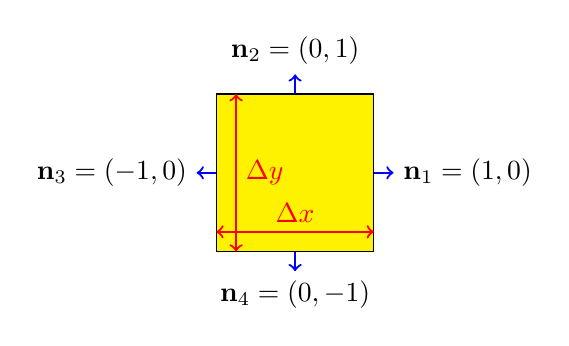
\begin{tikzpicture}[scale = 0.5]
\draw [fill=yellow] (0, 0) rectangle (4,4);
\node [right, red] at (0.5,2) {$\Delta y$};
\node [above, red] at (2,0.5) {$\Delta x$};
\draw [thick, red, <->] (0.5,0) -- (0.5,4);
\draw [thick, red, <->] (0, 0.5) -- (4, 0.5);
\draw [thick, blue, ->] (4,2) -- (4.5,2);
\node [right] at (4.5,2) {$\mathbf{n}_{1}=(1,0)$};

\draw [thick, blue, ->] (2,4) -- (2,4.5);
\node [above] at (2,4.5) {$\mathbf{n}_{2}=(0,1)$};

\draw [thick, blue, ->] (0,2) -- (-0.5,2);
\node [left] at (-0.5,2) {$\mathbf{n}_{3}=(-1,0)$};

\draw [thick, blue, ->] (2,0) -- (2,-0.5);
\node [below] at (2,-0.5) {$\mathbf{n}_{4}=(0,-1)$};
\end{tikzpicture}
\caption{Viscous diffusion}
\label{fig:stagg_diffusion}
\end{figure}

where we can approximate the integral as

\begin{align}
\nu\oint_{S}\nabla u\cdot \hat{n}\ \text{d}S &= \nu\oint_{S}\left(\frac{\partial u}{\partial x}n_{x} + \frac{\partial u}{\partial y}n_{y}\right)\ \text{d}S\\
&\approx \nu\left[ \left.\frac{\partial u}{\partial x}\right|_{1}h + \left.\frac{\partial u}{\partial y}\right|_{2}h - \left.\frac{\partial u}{\partial x}\right|_{3}h - \left.\frac{\partial u}{\partial y}\right|_{4}h \right]\\
&\approx \nu\left[ \left.\frac{\partial u}{\partial x}\right|_{i+1,j}^{(n)} + \left.\frac{\partial u}{\partial y}\right|_{i,j}^{(n)} - \left.\frac{\partial u}{\partial x}\right|_{i+\frac{1}{2},j+\frac{1}{2}}^{(n)} - \left.\frac{\partial u}{\partial y}\right|_{i+\frac{1}{2},j-\frac{1}{2}}^{(n)} \right]h
\intertext{which if we discritize gives us the final result of}
\nu\oint_{S}\nabla u\cdot \hat{n}\ \text{d}S &\approx \nu\left(u_{i+\frac{3}{2},j}^{(n)} + u_{i-\frac{1}{2},j}^{(n)} + u_{i+\frac{1}{2},j+1}^{(n)} + u_{i+\frac{1}{2},j-1}^{(n)} - 4u_{i+\frac{1}{2},j}^{(n)}\right)
\intertext{and similiarly for the $y$-diffusion momentum gives}
\nu\oint_{S}\nabla v\cdot \hat{n}\ \text{d}S &\approx \nu\left( v_{i,j+\frac{3}{2}}^{(n)} + v_{i,j-\frac{1}{2}}^{(n)} + v_{i+1,j+\frac{1}{2}}^{(n)} + v_{i-1,j+\frac{1}{2}}^{(n)} - 4v_{i,j+\frac{1}{2}}^{(n)}\right)
\end{align}

\noindent{\bf  Combining Conservation Equations}

By combining the above conservation equations gives

\begin{align}
\frac{\partial}{\partial t} \int_{V}u\ \text{d}V &= -\oint_{S}u\vec{u}\cdot \hat{n}\ \text{d}S + \nu\oint_{S}\nabla u\cdot \hat{n}\ \text{d}S - \frac{1}{\rho}\oint_{S} pn_{x}\ \text{d}S
\intertext{where we can set $P = \frac{p}{\rho}$, making it}
\frac{\partial}{\partial t} \int_{V}u\ \text{d}V &= -\oint_{S}u\vec{u}\cdot \hat{n}\ \text{d}S + \nu\oint_{S}\nabla u\cdot \hat{n}\ \text{d}S - \oint_{S} Pn_{x}\ \text{d}S
\end{align}

where we can discritize this with the above equations that were defined.

\noindent{\bf  Description of Solution Technique}

The above momentum equations can be rewritten as a single vector equation

\begin{align}
\frac{\vec{u}_{i,j}^{(n+1)}-\vec{u}_{i,j}^{(n)}}{\Delta t} &= -\vec{A}_{i,j}^{(n)} - \nabla P_{i,j} + \vec{D}_{i,j}^{(n)}\label{eq:vel}
\intertext{with $\vec{A}$ being the advection term, and $\vec{D}$ being the diffusiveness term. The mass conservation equations can be written as a {\em constraint} for our velocity update which is}
\nabla \cdot \vec{u}_{i,j}^{(n+1)} &= 0\label{eq:vel_constraint}
\intertext{where Equation~\ref{eq:vel} can be used as the Evolution of the velocity. However, there is no explicit equation for the velocity, but can be solved in the following way. We can split Equation~\ref{eq:vel} into}
\frac{\vec{u}_{i,j}^{(t)}-\vec{u}_{i,j}^{(n)}}{\Delta t} &= -\vec{A}_{i,j}^{(n)} + \vec{D}_{i,j}^{(n)}\Rightarrow \vec{u}_{i,j}^{(t)} = \vec{u}_{i,j}^{(n)} + \Delta t \left(-\vec{A}_{i,j}^{(n)} + \vec{D}_{i,j}^{(n)}\right)\\
\intertext{and}
\frac{\vec{u}_{i,j}^{(n+1)} - \vec{u}_{i,j}^{(t)}}{\Delta t} &= -\nabla P_{i,j} \Rightarrow \vec{u}_{i,j}^{(n+1)} = \vec{u}_{i,j}^{(t)} - \Delta t \nabla P_{i,j}\label{eq:vel_new}
\intertext{where a temporary velocity $\vec{u}^{(t)}$ was introduced to split the equation. To derive the equation for Pressure, we can take the divergence of \ref{eq:vel_new}, and with the constraint given in Equation~\ref{eq:vel_constraint} gives}
\cancel{\nabla \cdot \vec{u}_{i,j}^{(n+1)}} &= \nabla \cdot \vec{u}_{i,j}^{(t)} - \Delta t \nabla \cdot \nabla P_{i,j}\\
\Rightarrow \nabla ^{2}P_{i,j} &= \frac{1}{\Delta t}\nabla \cdot \vec{u}_{i,j}^{(t)}
\end{align}

which now gives us all the equations that we need to solve the system of equations. To solve the system, we take the following steps:

\begin{enumerate}
\item Impose Boundary Conditions
\item Find a temporary velocity using the advection and the diffusion terms only
\begin{align}
\vec{u}_{i,j}^{(t)} &= \vec{u}_{i,j}^{(n)} + \Delta t \left( - \vec{A}_{i,j}^{(n)} + \vec{D}_{i,j}^{(n)}\right)
\end{align}
\item Find the pressure needed to make the velocity field incompressible
\begin{align}
\nabla^{2} P^{(n+1)}_{i,j} &= \frac{1}{\Delta t}\nabla \cdot \vec{u}_{i,j}^{(t)}
\end{align}
\item Correct the velocity by adding the pressure gradient
\begin{align}
\vec{u}_{i,j}^{(n+1)} &= \vec{u}_{i,j}^{(t)} - \Delta t \nabla P_{i,j}\label{eq:vel_corr}
\end{align}
\item Return to 1 if $\left|\left| P^{(n+1)} - P^{(n)}\right|\right|_{2} > \text{tolerance}$
\end{enumerate}

\noindent{\bf  Solving the Pressure Equation}

We can get the equation for the pressure by taking Equation~\ref{eq:vel_corr} and plugging it into Equation~\ref{eq:vel_constraint} after discritizing gives us:

\begin{align}
&P_{i+1,j} + P_{i-1,j} + P_{i,j+1} + P_{i,j-1} - 4P_{i,j} =\nonumber\\
&\frac{h}{\Delta t} \left( u_{i+\frac{1}{2},j}^{(t)} - u^{(t)}_{i-\frac{1}{2},j} + v^{(t)}_{i,j+\frac{1}{2}} - v^{(t)}_{i,j-\frac{1}{2}}\right)
\end{align}
where, solving for $P_{i,j}$ gives
\begin{align}
P_{i,j} &= \frac{1}{4}\left[ \left(P_{i+1,j} + P_{i-1,j} + P_{i,j+1} + P_{i,j-1}\right) \right.\nonumber\\
&\left. - \frac{h}{\Delta t} \left( u_{i,j}^{(t)} - u_{i-1,j}^{(t)} + v_{i,j}^{(t)}-v_{i,j-1}^{(t)}\right)\right]
\end{align}

\noindent{\bf  Vorticity}

The voriticy of the system can be calculated as

\begin{align}
\omega &= \frac{\text{d}v}{\text{d}x} - \frac{\text{d}u}{\text{d}y}
\end{align}

\end{document}
